\documentclass[14pt,a4paper]{extarticle}

\usepackage{fontspec}
\usepackage[russian]{babel}
\setmainfont{Times New Roman}
\setsansfont{Arial}
\setmonofont{Times New Roman}[Scale=1]

\usepackage[left=30mm,right=15mm,top=20mm,bottom=20mm]{geometry}
\usepackage{setspace}
\usepackage{indentfirst}
\usepackage{amsmath}
\usepackage{booktabs}
\usepackage{hhline}
\usepackage{longtable}
\usepackage{array}
\usepackage{tabularx}
\usepackage{enumitem}
\usepackage{listings}
\usepackage{xcolor}
\usepackage{tikz}
\usepackage{pgfplots}
\pgfplotsset{compat=1.18}
\usepackage{float}
\usepackage{caption}
\usepackage{pdfpages}
\usepackage{pdflscape}
\usepackage{hyperref}
\usepackage{titlesec}
\urlstyle{same}

\addto\captionsrussian{\renewcommand{\contentsname}{СОДЕРЖАНИЕ}}

\usetikzlibrary{arrows.meta,positioning,shapes.geometric}

\onehalfspacing
\setlength{\parindent}{1.25cm}
\setlength{\parskip}{0pt}
\setlength{\emergencystretch}{3em}
\hyphenpenalty=10000
\exhyphenpenalty=10000
\sloppy
\clubpenalty=10000
\widowpenalty=10000
\displaywidowpenalty=10000
\setlength{\rightskip}{0.5mm}
\AtBeginDocument{%
    \setlength{\abovedisplayskip}{0pt}%
    \setlength{\abovedisplayshortskip}{0pt}%
    \setlength{\belowdisplayskip}{0pt}%
    \setlength{\belowdisplayshortskip}{0pt}%
}
\hypersetup{
    hidelinks,
    pdftitle={Сравнительный анализ ресурсной эффективности алгоритмов},
    pdfauthor={Ананьев Никита Андреевич}
}

\setlist[itemize]{
    label=---,
    labelindent=\parindent,
    leftmargin=*,
    nosep
}
\setlist[enumerate]{
    label=\arabic*),
    labelindent=\parindent,
    leftmargin=*,
    nosep
}

\titleformat{\section}[hang]
    {\normalfont\Large\bfseries\raggedright\hyphenpenalty=10000\exhyphenpenalty=10000}
    {\hspace*{1.25cm}\thesection}{\fontdimen2\font}{}
\titleformat{name=\section,numberless}[block]
    {\normalfont\Large\bfseries\centering\hyphenpenalty=10000\exhyphenpenalty=10000}
    {}{0pt}{}
\titleformat{\subsection}[hang]
    {\normalfont\large\bfseries\raggedright\hyphenpenalty=10000\exhyphenpenalty=10000}
    {\hspace*{1.25cm}\thesubsection}{\fontdimen2\font}{}
\titlespacing*{\section}{0pt}
    {0pt}{2.3ex plus .2ex}
\titlespacing*{\subsection}{0pt}
    {3.25ex plus 1ex minus .2ex}{1.5ex plus .2ex}

\newcommand{\structuralpart}[1]{%
    \clearpage
    \section*{#1}%
    \phantomsection
    \addcontentsline{toc}{section}{#1}%
}

\captionsetup{labelsep=endash}
\captionsetup[figure]{name=Рисунок,justification=centering}
\captionsetup[table]{name=Таблица,justification=raggedright,
    singlelinecheck=false,skip=2pt}
\setlength{\doublerulesep}{0.5pt}

\makeatletter
\renewcommand{\tagform@}[1]{%
    \maketag@@@{\kern1mm(\ignorespaces#1\unskip\@@italiccorr)\kern1mm}}
\renewcommand{\@biblabel}[1]{#1.}
\renewenvironment{thebibliography}[1]
    {\section*{\refname}%
     \@mkboth{\MakeUppercase\refname}{\MakeUppercase\refname}%
     \list{\@biblabel{\@arabic\c@enumiv}}%
          {\settowidth\labelwidth{\@biblabel{#1}}%
           \leftmargin\z@
           \itemindent\dimexpr\parindent+\labelwidth+\labelsep\relax
           \rightmargin 5mm
           \@openbib@code
           \usecounter{enumiv}%
           \let\p@enumiv\@empty
           \renewcommand\theenumiv{\@arabic\c@enumiv}}%
     \sloppy
     \clubpenalty4000
     \@clubpenalty\clubpenalty
     \widowpenalty4000
     \sfcode`\.\@m}
    {\def\@noitemerr
         {\@latex@warning{Empty `thebibliography' environment}}%
     \endlist}
\renewcommand*\l@section[2]{%
    \ifnum\c@tocdepth>\z@
        \addpenalty\@secpenalty
        \addvspace{.5em \@plus\p@}%
        \setlength\@tempdima{\dimexpr\parindent+1.5em\relax}%
        \begingroup
        \parindent\z@ \rightskip\@pnumwidth
        \parfillskip-\@pnumwidth
        \leavevmode\bfseries
        \advance\leftskip\@tempdima
        \hskip-\leftskip
        \hspace*{1.25cm}%
        #1\nobreak\hfil\nobreak
        \hb@xt@\@pnumwidth{\hss #2}\par
        \endgroup
    \fi}
\renewcommand*\l@subsection[2]{%
    \@dottedtocline{2}{1.25cm}{2.8em}{#1}{#2}}
\makeatother

\lstset{
    basicstyle=\normalfont\normalsize\rmfamily\setstretch{1},
    keywordstyle=\color{black},
    commentstyle=\color{black},
    stringstyle=\color{black},
    numbers=left,
    numberstyle=\normalfont\normalsize\rmfamily,
    stepnumber=1,
    numbersep=5pt,
    xleftmargin=9mm,
    linewidth=\dimexpr\linewidth-9mm\relax,
    frame=single,
    breaklines=true,
    columns=fullflexible,
    keepspaces=true,
    showstringspaces=false,
    tabsize=4
}
\renewcommand{\lstlistingname}{Листинг}

\tikzset{
    algorithm block/.style={draw,align=center,minimum width=64mm,
        inner xsep=0pt,inner ysep=2pt},
    terminator/.style={algorithm block,rectangle,rounded corners=5mm,
        minimum height=10mm},
    data/.style={trapezium,trapezium left angle=70,
        trapezium right angle=110,trapezium stretches=true,
        algorithm block,text width=54mm,minimum height=10mm},
    process/.style={algorithm block,rectangle,text width=54mm,
        minimum height=10mm},
    decision/.style={diamond,draw,align=center,aspect=3.2,
        minimum width=64mm,minimum height=20mm,inner sep=0pt},
    loop start/.style={rectangle,align=center,draw=none,
        minimum width=64mm,minimum height=12mm,text width=54mm,
        inner xsep=0pt,inner ysep=2pt,path picture={
            \draw[black]
                ([yshift=-5mm]path picture bounding box.north west) --
                ([xshift=5mm]path picture bounding box.north west) --
                ([xshift=-5mm]path picture bounding box.north east) --
                ([yshift=-5mm]path picture bounding box.north east) --
                (path picture bounding box.south east) --
                (path picture bounding box.south west) -- cycle;
        }},
    loop end/.style={rectangle,align=center,draw=none,
        minimum width=64mm,minimum height=12mm,text width=54mm,
        inner xsep=0pt,inner ysep=2pt,path picture={
            \draw[black]
                (path picture bounding box.north west) --
                (path picture bounding box.north east) --
                ([yshift=5mm]path picture bounding box.south east) --
                ([xshift=-5mm]path picture bounding box.south east) --
                ([xshift=5mm]path picture bounding box.south west) --
                ([yshift=5mm]path picture bounding box.south west) -- cycle;
        }},
    flow/.style={draw,-{Latex[length=2.5mm]}},
    every node/.style={font=\small}
}

\hypersetup{pdftitle={Лабораторная работа № 5. Конвейерная обработка изображений},pdfauthor={Понарин А. А.}}
\setcounter{tocdepth}{2}
\AtBeginDocument{\hyphenpenalty=85\exhyphenpenalty=85\setlength{\rightskip}{0pt}}
\newcommand{\TimeRows}{%
512 & 1 & 1{,}48 & 1{,}81 & 0{,}82 \\\hline%
512 & 4 & 6{,}74 & 10{,}99 & 0{,}61 \\\hline%
512 & 16 & 30{,}23 & 52{,}91 & 0{,}57 \\\hline%
512 & 32 & 80{,}56 & 97{,}35 & 0{,}83 \\\hline%
2048 & 1 & 10{,}78 & 11{,}19 & 0{,}96 \\\hline%
2048 & 4 & 40{,}47 & 29{,}37 & 1{,}38 \\\hline%
2048 & 16 & 159{,}12 & 112{,}63 & 1{,}41 \\\hline%
2048 & 32 & 403{,}44 & 349{,}34 & 1{,}15 \\\hline%
}

\newcommand{\StageRows}{%
512 & 0{,}29 & 0{,}42 & 1{,}35 & 14{,}41 \\\hline%
2048 & 3{,}18 & 7{,}60 & 4{,}58 & 65{,}75 \\\hline%
}

\lstset{language=C,basicstyle=\small\ttfamily\setstretch{1},numberstyle=\small,captionpos=b}
\tikzset{
  opbox/.style={process,minimum width=58mm,text width=52mm,font=\small},
  endstep/.style={terminator,minimum width=31mm,minimum height=8mm,font=\small},
  check/.style={decision,minimum width=44mm,minimum height=13mm,aspect=2.8,font=\small},
  lane/.style={draw,rectangle,align=center,minimum height=10mm,text width=20mm,font=\small},
  pipequeue/.style={lane,text width=12mm,dashed}
}

\begin{document}
\begin{titlepage}
\thispagestyle{empty}
\noindent\begin{minipage}[c]{0.15\textwidth}

\includegraphics[width=\linewidth]{shared/b_logo.jpg}
\end{minipage}\hfill
\begin{minipage}[c]{0.83\textwidth}\centering\small
Министерство науки и высшего образования Российской Федерации\\
Федеральное государственное автономное образовательное учреждение\\
высшего образования\\
«Московский государственный технический университет\\
имени Н.~Э.~Баумана\\
(национальный исследовательский университет)»\\
(МГТУ им. Н.~Э.~Баумана)
\end{minipage}
\par\vspace{4mm}\noindent\rule{\dimexpr\linewidth-1mm\relax}{1pt}\par\vspace{10mm}
\noindent ФАКУЛЬТЕТ «Информатика и системы управления»\\[4mm]
КАФЕДРА «Программная инженерия»
\vspace{23mm}
\begin{center}\Large\bfseries Лабораторная работа № 5\\[3mm]
по дисциплине «Анализ алгоритмов»\end{center}
\vspace{17mm}
\noindent Тема: «Конвейерная сегментация полутоновых изображений»
\par\vspace{15mm}
\noindent Студент: Понарин А.~А.\\[4mm]
Группа: ИУ7-55Б\\[4mm]
Преподаватели: Волкова Л.~Л., Строганов Д.~В.
\vfill\begin{center}2026~г.\end{center}
\end{titlepage}
\setcounter{page}{2}
\clearpage\tableofcontents

\structuralpart{ВВЕДЕНИЕ}
При обработке пакета изображений чтение файла, обработка пикселей и запись результата для одной заявки выполняются в заданном порядке. Заявки независимы друг от друга, поэтому чтение очередного файла можно совмещать с вычислениями и записью результатов предыдущих заявок.

Цель работы --- разработать трёхступенчатый конвейер сегментации изображений и оценить его влияние на время обработки пакета. Для этого поставлены следующие задачи.
\begin{enumerate}
\item определить состав заявки и операции каждого этапа;
\item разработать схемы последовательной и конвейерной обработки, реализовать передачу заявок между этапами;
\item проверить совпадение результатов и обработку ошибок;
\item измерить реальное время обработки пакетов, построить временную диаграмму и сравнить режимы.
\end{enumerate}

\clearpage\section{Аналитическая часть}
\subsection{Постановка задачи}
Генератор создаёт по заявке на каждое имя во входном списке и присваивает ей номер. За каждым обслуживающим устройством (ОУ) закреплена своя операция.
\begin{enumerate}
\item ОУ 1 считывает из указанного файла размеры и пиксели изображения в заявку;
\item ОУ 2 выполняет сегментацию методом Оцу, выбранным в ЛР4;
\item ОУ 3 записывает бинарную маску в отдельный файл.
\end{enumerate}
По номеру заявки определяется имя выходного файла. При повторении входного имени номера различаются. Ошибка заявки фиксируется в журнале, обработка остальных продолжается.

Файл содержит одно изображение PGM P5~\cite{pgm} с максимальной яркостью 255. При ширине \(W>0\) и высоте \(H>0\) растр занимает \(N=WH\) байт. После максимальной яркости следует один пробельный байт, затем растр. Маска имеет исходные размеры и значения 0 и 255.

\subsection{Сегментация методом Оцу}
Алгоритм строит гистограмму \(h_v\) для \(L=256\) уровней яркости, затем перебирает пороги \(t\) от 0 до 254. Для каждого порога вычисляются число и сумма яркостей пикселей тёмного класса, а также общая сумма яркостей:
\begin{equation}
  n_0(t)=\sum_{v=0}^{t}h_v,\qquad
  s_0(t)=\sum_{v=0}^{t}v h_v,\qquad
  s=\sum_{v=0}^{255}v h_v .
\end{equation}
Размер светлого класса равен \(n_1=N-n_0\). Если оба класса непусты, вычисляется критерий
\begin{equation}
  J(t)=\frac{(N s_0(t)-n_0(t)s)^2}{n_0(t)n_1(t)} .
\end{equation}
Критерий пропорционален межклассовой дисперсии~\cite{otsu}. \(n_0\) и \(s_0\) обновляются при переходе к следующему уровню. Из равных максимумов выбирается первый. Для однотонного входа порог равен яркости изображения. ОУ 2 записывает в тот же буфер 255 для яркостей выше порога и 0 для остальных.

\clearpage\section{Конструкторская часть}
\subsection{Организация конвейера}
Генератор работает в основном потоке. Три рабочих потока обслуживают очереди \(Q_1,Q_2,Q_3\) в порядке поступления заявок. В каждую очередь передаётся указатель на заявку. Поток извлекает заявку, выполняет свою операцию и передаёт её дальше. После ОУ 3 статус, порог и временные метки остаются в массиве заявок для последующего формирования журнала. Структура взаимодействия приведена на рисунке~\ref{fig:structure}.

\begin{figure}[H]\centering
\begin{tikzpicture}[node distance=2mm]
\node[lane,text width=20mm] (gen) {Генератор};
\node[pipequeue,right=of gen] (q1) {\(Q_1\)};
\node[lane,right=of q1] (read) {ОУ 1\\ Чтение};
\node[pipequeue,right=of read] (q2) {\(Q_2\)};
\node[lane,right=of q2] (compute) {ОУ 2\\ Оцу};
\node[pipequeue,right=of compute] (q3) {\(Q_3\)};
\node[lane,right=of q3] (write) {ОУ 3\\ Запись};
\foreach \a/\b in {gen/q1,q1/read,read/q2,q2/compute,compute/q3,q3/write}
  \draw[flow] (\a) -- (\b);
\node[lane,text width=31mm,below=of write] (files) {Файлы масок};
\draw[flow] (write) -- (files);
\end{tikzpicture}
\caption{Передача заявок между этапами}\label{fig:structure}
\end{figure}

Каждая очередь имеет два места, хранит индекс первого элемента и число занятых мест. При заполнении очереди сопровождающий её производитель ждёт свободного места. Потребитель спит, пока очередь открыта и пуста. Мьютекс защищает состояние очереди, а две условные переменные служат для уведомления о данных и свободном месте. Условие ожидания проверяется в цикле. Чтение, сегментация и запись выполняются после освобождения мьютекса.

Основной поток закрывает \(Q_1\) после передачи последней заявки. Закрытие разрешает ОУ 1 завершиться после опустошения очереди. Оно затем закрывает \(Q_2\), ОУ 2 аналогично закрывает \(Q_3\). Основной поток ожидает завершения всех рабочих и только затем обращается к итоговым данным. Если создать все потоки не удаётся, генерация не начинается: закрываются инициализированные очереди, затем ожидается завершение уже созданных потоков.

\clearpage\subsection{Схемы алгоритмов потоков}
В последовательном режиме операции одной заявки выполняются подряд в основном потоке. В конвейерном режиме основной поток передаёт заявки рабочим через \(Q_1\). Алгоритмы основных потоков приведены на рисунке~\ref{fig:main}.

\begin{figure}[H]\centering
\begin{tikzpicture}[node distance=5mm]
\node[font=\small\bfseries] (st) at (0,0) {Последовательный режим};
\node[endstep,below=of st] (s1) {Начало};
\node[opbox,below=of s1] (s2) {Создать заявки};
\node[check,below=of s2] (s3) {Есть заявка?};
\node[opbox,below=of s3] (s4) {Чтение, Оцу и запись\\для очередной заявки};
\node[opbox,below=8mm of s4] (s5) {Сформировать журнал};
\node[endstep,below=of s5] (s6) {Конец};
\draw[flow] (s1) -- (s2);
\draw[flow] (s2) -- (s3);
\draw[flow] (s3) -- node[right] {да} (s4);
\draw[flow] (s4.west) -- ++(-3mm,0) |- (s3.west);
\draw[flow] (s3.east) -- ++(9mm,0) node[above] {нет} |- (s5.east);
\draw[flow] (s5) -- (s6);

\node[font=\small\bfseries] (pt) at (8.15,0) {Конвейерный режим};
\node[endstep,below=of pt] (p1) {Начало};
\node[opbox,below=of p1] (p2) {Создать заявки, очереди\\и рабочие потоки};
\node[check,below=of p2] (p3) {Есть заявка?};
\node[opbox,below=of p3] (p4) {Передать очередную\\заявку в \(Q_1\)};
\node[opbox,below=8mm of p4] (p5) {Закрыть \(Q_1\), дождаться\\рабочих, сохранить журнал};
\node[endstep,below=of p5] (p6) {Конец};
\draw[flow] (p1) -- (p2);
\draw[flow] (p2) -- (p3);
\draw[flow] (p3) -- node[right] {да} (p4);
\draw[flow] (p4.west) -- ++(-3mm,0) |- (p3.west);
\draw[flow] (p3.east) -- ++(9mm,0) node[above] {нет} |- (p5.east);
\draw[flow] (p5) -- (p6);
\end{tikzpicture}

\caption{Схемы основных потоков последовательного и конвейерного режимов}\label{fig:main}
\end{figure}

\clearpage
Для трёх рабочих потоков используется общий цикл (рисунок~\ref{fig:worker}). Его операция определяется номером ОУ. На каждом этапе сохраняются метки начала и окончания выполненной операции.

\begin{figure}[H]\centering
\begin{tikzpicture}[node distance=5mm]
\node[endstep] (start) {Начало};
\node[opbox,below=of start] (pop) {Извлечь заявку. Ждать,\\пока очередь открыта и пуста};
\node[check,below=of pop] (found) {Есть заявка?};
\node[opbox,below=of found] (operation) {Выполнить операцию ОУ,\\если у заявки нет ошибки};
\node[opbox,below=of operation] (forward)
  {Передать заявку дальше\\или завершить обработку\\и освободить буфер};
\node[opbox,right=16mm of found,text width=36mm,minimum width=40mm] (close)
  {Закрыть выходную очередь,\\если она есть};
\node[endstep,below=of close] (end) {Конец};
\draw[flow] (start) -- (pop);
\draw[flow] (pop) -- (found);
\draw[flow] (found) -- node[right] {да} (operation);
\draw[flow] (operation) -- (forward);
\draw[flow] (forward.west) -- ++(-5mm,0) |- (pop.west);
\draw[flow] (found) -- node[above] {нет} (close);
\draw[flow] (close) -- (end);
\end{tikzpicture}

\caption{Схема алгоритма рабочего потока}\label{fig:worker}
\end{figure}

\begin{table}[H]\caption{Действия рабочих потоков}\label{tab:devices}
\centering
\begin{tabularx}{\textwidth}{|l|>{\raggedright\arraybackslash}X|>{\raggedright\arraybackslash}X|}\hline
Поток & Вход и операция & Действие после операции\\\hline
ОУ 1 & Имя файла. Чтение заголовка и растра PGM &
В \(Q_2\) поступает заявка с буфером или с кодом ошибки.\\\hline
ОУ 2 & Буфер яркостей. Гистограмма, выбор порога, замена яркостей на байты маски &
В \(Q_3\) поступает заявка с порогом и маской. Заявка с ошибкой передаётся без вычислений.\\\hline
ОУ 3 & Размеры и буфер маски. Запись временного файла и переименование &
Маска сохраняется под номером заявки. Буфер освобождается, итог остаётся в массиве.\\\hline
\end{tabularx}
\end{table}

\clearpage\subsection{Корректность и оценки затрат}
Заявка с номером \(i\) помещается в \(Q_1\) ровно один раз. Каждая очередь передаёт её единственному потребителю, а блокировка очереди обеспечивает видимость изменений, сделанных перед передачей. Опустошение закрытой очереди предшествует закрытию следующей. Следовательно, при штатном завершении каждая заявка доходит до ОУ 3 ровно один раз, а очереди сохраняют порядок номеров. Оба режима используют одинаковые операции над одной заявкой и формируют одинаковые маски при одинаковых входных данных.

При \(M\) заявках и \(N_i\) пикселях в заявке \(i\) построение гистограммы, обход порогов и бинаризация требуют \(O(N_i+L)\) действий. Файловые операции обрабатывают по \(N_i\) байт растра. Суммарная алгоритмическая работа обоих режимов составляет \(O(\sum_{i=1}^{M}(N_i+L))\) при ограниченной длине имён и заголовков. Операции с кольцевым буфером требуют \(O(1)\) действий без времени ожидания.

В \(Q_1\) лежат заявки с именами файлов. Буферы пикселей могут находиться в \(Q_2,Q_3\) и у трёх рабочих, то есть одновременно их не более семи. При \(N_{\max}=\max_i N_i\) последовательный режим хранит один буфер, конвейерный --- до семи, а массив метаданных в каждом режиме занимает \(O(M)\). На гистограмму приходится \(O(L)\) дополнительной памяти.

При одинаковых длительностях соответствующих операций для всех заявок, отсутствии издержек передачи и конкуренции за ресурсы время одного заказа равно сумме \(s_1+s_2+s_3\). Идеальное время пакета из \(M\) заявок описывается выражением
\begin{equation}
  T_{\text{конв}}=s_1+s_2+s_3+(M-1)\max(s_1,s_2,s_3).
\end{equation}
После заполнения конвейера темп выпуска задаёт самый медленный этап. Реальное время зависит также от планирования потоков, заполненности очередей и работы файловой системы.

\clearpage\section{Технологическая часть}
\subsection{Средства реализации и интерфейс}
Программа написана на C11. GCC собирает её с библиотекой POSIX Threads, на Windows используется пакет GCC MSYS2 UCRT64. Реализация очерёдности и обработки заявок находится в файле \texttt{src/pipeline.c}, чтение PGM, сегментация и запись --- в \texttt{src/image.c}, интерфейс и журналирование --- в \texttt{src/main.c}. Фрагмент реализации рабочего потока приведён в приложении~А.

\noindent Пример запуска из каталога лабораторной работы приведён ниже.
\begin{lstlisting}[numbers=none]
.\lab5.exe seq  seq_out input.pgm input.pgm
.\lab5.exe pipe pipe_out input.pgm input.pgm
\end{lstlisting}

Выходной каталог создаётся при запуске. Для приведённого примера в нём появятся две маски \texttt{000001.pgm}, \texttt{000002.pgm} и журнал \texttt{trace.csv}. В журнале номер соответствует позиции имени в командной строке. Для каждой заявки сохраняются статус, порог, момент отправки и интервалы реально выполненных операций. Если файл не открывается или растр некорректен, вычисление и запись для этой заявки пропускаются. Ошибка отражается в журнале и в коде завершения программы. При ошибке записи временный файл удаляется.

\clearpage\subsection{Функциональная проверка}
Функциональные тесты выполнены в обоих режимах для одиночной заявки, пакета корректных изображений и пакета с ошибочными файлами. Рассчитаны 84 маски и проверена обработка 12 ошибочных заявок. Эталон рассчитывает критерий с рациональными числами. С эталоном сверялись пороги, размеры и байты записанных масок. Примеры приведены в таблице~\ref{tab:tests}.

\begin{table}[H]\caption{Примеры функциональных проверок}\label{tab:tests}
\centering
\begin{tabularx}{\textwidth}{|>{\raggedright\arraybackslash}X|>{\raggedright\arraybackslash}X|}\hline
Вход & Полученный результат\\\hline
15 пикселей яркости 77 & Порог 77, 15 нулей\\\hline
\((10,10,200,200)\) & Порог 10, маска \((0,0,255,255)\)\\\hline
\((0,2,4)\) & Порог 0 при равенстве критерия, маска \((0,255,255)\)\\\hline
Все яркости от 0 до 255 & Порог 127, 128 нулей и 128 значений 255\\\hline
Нет файла, усечённый или лишний байт растра & Статус ошибки, файл маски отсутствует\\\hline
Повтор одного имени в пакете & Побайтно равные маски в файлах с разными номерами\\\hline
\end{tabularx}
\end{table}

Также проверены хронология этапов по журналу, последовательность номеров, продолжение работы после ошибки и защита существующего выходного каталога.

\clearpage\section{Исследовательская часть}
\subsection{Условия и методика замеров}
Замеры выполнены на Intel Core i3-1115G4 с четырьмя логическими процессорами под Windows 11, сборка 26200. Использован GCC 14.2.0 с опцией \texttt{-O2}. Реальное время измерено через \texttt{QueryPerformanceCounter}~\cite{timer}. В интервал входят подготовка массива заявок, запуск и завершение рабочих, работа очередей, файловые операции и сегментация. Создание выходного каталога, сохранение журнала и подготовка входных файлов выполняются вне интервала.

Исследованы пакеты из \(M\in\{1,4,16,32\}\) заявок на изображениях \(512\times512\) и \(2048\times2048\). Для каждого размера создано четыре файла с псевдослучайными яркостями. При составлении пакета имена выбираются циклически, оба режима получают одинаковый список. Для каждой конфигурации выполнены один прогрев и 15 измерений каждого режима с чередованием порядка запуска. Всего учтено 240 измерений. В исследовании действовало штатное кэширование файловой системы, принудительная синхронизация записи с накопителем не выполнялась.

\clearpage\subsection{Время обработки пакета}
В таблице~\ref{tab:times} представлены медианные времена пакета. Ускорение \(S\) рассчитано как отношение медианы последовательного режима к медиане конвейерного. Вертикальные отрезки на рисунке~\ref{fig:times} показывают интервал от первого до третьего квартиля.

\begin{table}[H]\caption{Медианное время обработки пакета}\label{tab:times}
\centering
\begin{tabular}{|c|c|c|c|c|}\hline
Сторона, пикс. & Заявок & Послед., мс & Конвейер, мс & \(S\)\\\hline
\TimeRows
\end{tabular}
\end{table}

\begin{figure}[H]\centering
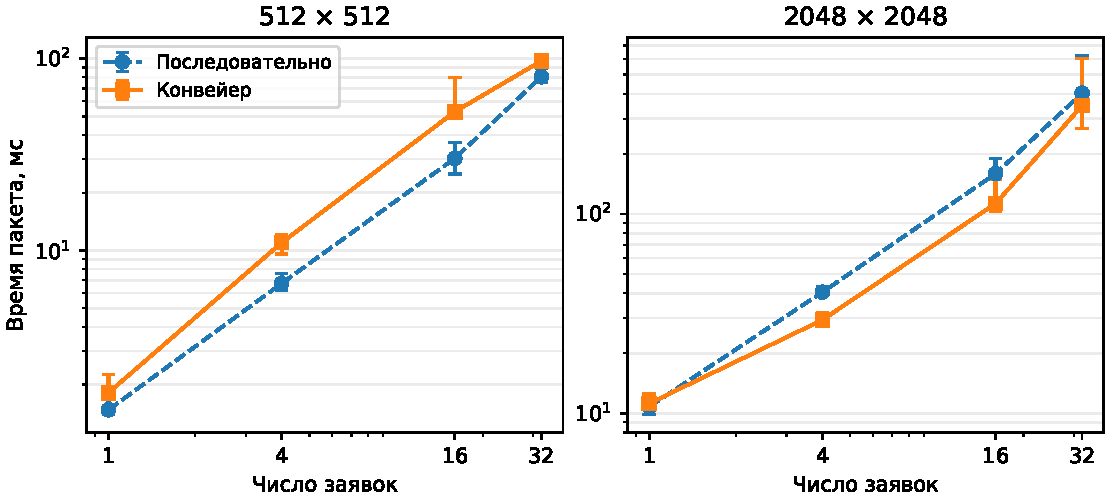
\includegraphics[width=\textwidth]{figures/times.pdf}
\caption{Зависимость времени обработки от числа заявок}\label{fig:times}
\end{figure}

\clearpage\subsection{Работа этапов и задержка заявки}
В таблице~\ref{tab:stages} приведены медианы по 15 прогонам. Длительности операций усреднялись по заявкам каждого прогона, для задержки бралась медиана. Задержка отсчитывается от попытки поместить заявку в \(Q_1\) до окончания записи маски.

\begin{table}[H]\caption{Медианные показатели конвейера для 32 заявок}\label{tab:stages}
\centering
\begin{tabular}{|c|c|c|c|c|}\hline
Сторона, пикс. & Чтение, мс & Оцу, мс & Запись, мс & Задержка, мс\\\hline
\StageRows
\end{tabular}
\end{table}

На рисунке~\ref{fig:timeline} показаны первые восемь заявок из пакета из 16 изображений \(2048\times2048\). Для каждого режима выбран прогон с медианным временем. Прямоугольники обозначают интервалы операций, числа внутри --- номера заявок. В конвейерном режиме интервалы разных заявок перекрываются.

\begin{figure}[H]\centering
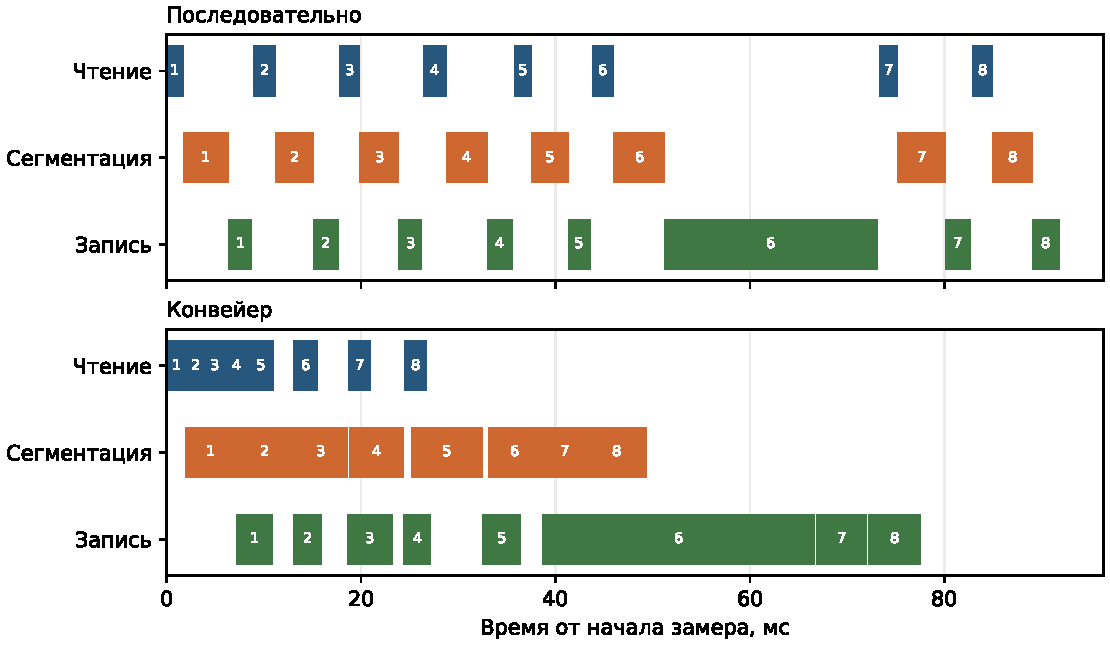
\includegraphics[width=\textwidth]{figures/timeline.pdf}
\caption{Измеренные интервалы выполнения операций для первых восьми заявок}\label{fig:timeline}
\end{figure}

\clearpage\subsection{Анализ результатов}
Для одной заявки совмещение этапов невозможно. При стороне 2048 медианы составили 10,78 мс в последовательном режиме и 11,19 мс в конвейерном. При стороне 512 конвейер уступил во всех измеренных конфигурациях. В частности, для 16 заявок получено 30,23 и 52,91 мс соответственно. Для пакета из 32 малых изображений запись занимала больше времени, чем чтение и сегментация вместе. Потенциал ускорения за счёт перекрытия этих коротких операций в такой конфигурации ограничен, а накладные расходы на обмен заявками, планирование потоков и совместное использование ресурсов входят в замер.

При стороне 2048 и \(M=4,16,32\) медиана конвейерного режима оказалась ниже. Наибольшее отношение медиан \(1{,}41\) получено для 16 заявок: время уменьшилось со 159,12 до 112,63 мс. Для 32 заявок получено ускорение \(1{,}15\), а межквартильные интервалы двух режимов существенно перекрылись. Поэтому выигрыш для этого размера пакета описывается по медианам и зависит от условий запуска.

При пакетах из 32 больших изображений самым длительным этапом конвейера по измеренным длительностям была сегментация (7,60 мс против 3,18 мс для чтения и 4,58 мс для записи). Медианная задержка заявки составила 65,75 мс, поскольку включает ожидание в очередях. Таким образом, ускорение обработки всего пакета может сопровождаться увеличением задержки отдельной заявки.

\structuralpart{ЗАКЛЮЧЕНИЕ}
Разработана трёхступенчатая обработка заявок с чтением файла, сегментацией методом Оцу и сохранением отдельной маски. Конвейер передаёт заявки через ограниченные очереди и сохраняет порядок обработки на каждом этапе. Результаты последовательного и конвейерного режимов совпали с независимым эталоном на всех корректных тестовых входах.

Временная диаграмма показала перекрытие операций над разными заявками. Для изображений \(2048\times2048\) и пакета из 16 заявок получено наибольшее медианное ускорение среди исследованных конфигураций, равное 1,41. Для изображений \(512\times512\) и для одиночных заявок в исследованных условиях последовательный режим имел меньшую медиану времени.


\clearpage
\renewcommand{\refname}{СПИСОК ИСПОЛЬЗОВАННЫХ ИСТОЧНИКОВ}
\phantomsection\addcontentsline{toc}{section}{СПИСОК ИСПОЛЬЗОВАННЫХ ИСТОЧНИКОВ}
\begin{thebibliography}{3}
\raggedright
\bibitem{pgm} Netpbm. PGM Format Specification. URL: \url{https://netpbm.sourceforge.net/doc/pgm.html} (дата обращения: 19.11.2026).
\bibitem{otsu} Otsu N. A Threshold Selection Method from Gray-Level Histograms // IEEE Transactions on Systems, Man, and Cybernetics. 1979. Vol.~9, no.~1. P.~62--66. DOI: \href{https://doi.org/10.1109/TSMC.1979.4310076}{10.1109/TSMC.1979.4310076}.
\bibitem{timer} Microsoft. QueryPerformanceCounter function. URL: \url{https://learn.microsoft.com/en-us/windows/win32/api/profileapi/nf-profileapi-queryperformancecounter} (дата обращения: 19.11.2026).
\end{thebibliography}

\structuralpart{ПРИЛОЖЕНИЕ А}
\begin{center}Фрагменты реализации\end{center}
В листинге~\ref{lst:fifo} приведена операция извлечения заявки из очереди. Она ожидает заявку, пока очередь открыта, и возвращает пустой указатель после опустошения закрытой очереди.
\lstinputlisting[caption={Извлечение заявки из очереди},label={lst:fifo},linerange={60-74},firstnumber=60]{src/pipeline.c}

В листинге~\ref{lst:worker} приведён цикл рабочего потока. После обработки заявки он передаёт её следующему устройству, а после завершения закрывает соответствующую очередь.
\lstinputlisting[caption={Общий цикл рабочего потока},label={lst:worker},linerange={110-123},firstnumber=110]{src/pipeline.c}
\end{document}
